%%%%%%%%%%%%%%%%%%%%%%%%%%%%%%%%%%%%%%%%%%%%%%%%%%%%%%%%%%%%%%%%%%%%%%
%%%%%%%%%%%%%%%%%%%%%%%%%%%%%%%%%%%%%%%%%%%%%%%%%%%%%%%%%%%%%%%%%%%%%%
\documentclass[dvips,portrait]{seminar}             %%%%%%%%%%%%%%%%%%
                                                    %%%%%%%%%%%%%%%%%%
%%%%%%%%%%%%%%%%%%%%%%%%%%%%%%%%%%%%%%%%%%%%%%%%%%%%
% (latex PairsKK+KW; dvips PairsKK+KW.dvi -o)
% (gv -bg white -fg black  -magstep -1  PairsKK+KW.ps&)
% pstops '1:0@0.925(10mm,-1mm)'  PairsKK+KW.ps   PairsKK+KW-redu.ps
%======================

%%%%%%%%%%%%%%%%%%%%%%%%%%%%%%%%%%%%%%%%%%%%%%%%%%%%%%%
%%%%%%%%%%%%%%%%%%%%%%%%%%%%%%%%%%%%%%%%%%%%%%%%%%%%%%%
\begin{document}                     %%%%%%%%%%%%%%%%%%


\def\title{\Color{PineGreen} Pairs KKMC+KoralW}

%%%%%%%%%%%%%%%%%%%%%%%%%%%%%%%%%%%%%%%%%%%%%%%%%%%%%%%%%%%%%%%%%%%%%%%%%%%%%
%%%%%%%%%%%%%%%%%%%%%%%%%%%%%%%%%%%%%%%%%%%%%%%%%%%%%%%%%%%%%%%%%%%%%%%%%%%%%
%%%%%%%%%%%%%%%%%%%%%%%%%%%%%%%%%%%%%%%%%%%%%%%%%%%%%%%%%%%%%%%%%%%%%%%%%%%%%
\begin{slide*}                                                %%%%%%%%%%%%%%%

\hbox{ }
\vspace{5mm}

\begin{center}
{\huge\color{red}\bf       Real+Virtual Pairs\\
                           from KKMC and KoralW}\\
\end{center}

\begin{center}
{\LARGE\color{red}          Very preliminary!}
\end{center}

\vspace{1mm}
\begin{center}
{\large\color{blue}\bf     Prepared by M. Skrzypek and S. Jadach}
\end{center}


\vspace{1mm}
\begin{center}
{\large\color{blue}\bf     To be presented by Z. W\c{a}s\\
	                   at EWG meeting, CERN June 6-th, 2000}
\end{center}

\vspace{2mm}
{\large\Color{PineGreen}\bf
OUTLINE:
\begin{itemize}
\item Itro: Kobel's proposal etc.
\item Virtual pairs in KKMC
\item Real pairs in KORALW
\item First numerical results
\item News from KKMC development
\end{itemize}
}

\vfill
\end{slide*}   %%%
%%%%%%%%%%%%%%%%%%


%%%%%%%%%%%%%%%%%%%%%%%%%%%%%%%%%%%%%%%%%%%%%%%%%%%%%%%%%%%%%%%%%%%%%%%%%%%%%
%%%%%%%%%%%%%%%%%%%%%%%%%%%%%%%%%%%%%%%%%%%%%%%%%%%%%%%%%%%%%%%%%%%%%%%%%%%%%
%%%%%%%%%%%%%%%%%%%%%%%%%%%%%%%%%%%%%%%%%%%%%%%%%%%%%%%%%%%%%%%%%%%%%%%%%%%%%
\begin{slide*}                                                %%%%%%%%%%%%%%%

{\bf Dictionary:}\\
{\Color{PineGreen} ISNS pairs} = Initial State Non-Singlet pairs\\
{\Color{PineGreen} FSNS pairs} = Final State Non-Singlet pairs\\
{\Color{PineGreen} ISNS$_{\gamma}$, ISNS$_{Z}$} = ISNS through $\gamma$ or $Z$ exchange.\\
{\Color{PineGreen} $2f$ Signal} = publishable exper. result., 
used to extract SM params, common for LEP2 collabs, 
based on Feynman diags.\\
{\Color{PineGreen} Efficiency} = 
Combined {\bf Theoretical} and {\bf Experimental} correction (detector eff. and cuts)
``real data'' $\to$ ``$2f$ Signal''.


{\Color{Blue} {\bf Michael Kobel proposes}: 
\fbox{Only ISNS$_{\gamma}$ $\in$ $2f$ Exper. Signal.}}

{\bf Consequences:}\\
{\Color{Red} 
(1) ISNS$_{\gamma}$ has to be in ZFITTER or other
semian. program representing the SM.
The ISNS$_{\gamma}$ part must be very well tested!\\
(2) $4f$ MC needed to subtracf the rest of $4f$, 
with the split in its matr. element:
$|{\cal M}^{4f}_{all.diagr.}|^2 = |{\cal M}^{4f}_{ISNS_{\gamma}}|^2$+BKG$^{4f}$.}

{\bf Advertized advantages:}\\
Mother Nature is responsible for cancellation of 
the virtual-real mass singularities (in the exper. data)
hence:\\
(A) No need of sophisticated MC$^{2f}$ $+$ MC$^{4f}$, :-)\\
(B) Only relatively crude MC$^{4f}$ needed for remooving total
    ``{\Color{PineGreen} Efficiency}'' which includes correction for BKG$^{4f}$
    ($\pm5\%$ prec.).
\vfill
\end{slide*}   %%%
%%%%%%%%%%%%%%%%%%

%%%%%%%%%%%%%%%%%%%%%%%%%%%%%%%%%%%%%%%%%%%%%%%%%%%%%%%%%%%%%%%%%%%%%%%%%%%%%
%%%%%%%%%%%%%%%%%%%%%%%%%%%%%%%%%%%%%%%%%%%%%%%%%%%%%%%%%%%%%%%%%%%%%%%%%%%%%
%%%%%%%%%%%%%%%%%%%%%%%%%%%%%%%%%%%%%%%%%%%%%%%%%%%%%%%%%%%%%%%%%%%%%%%%%%%%%
\begin{slide*}                                                %%%%%%%%%%%%%%%

{\Color{Blue}\bf Where are we?:}\\
(1) ISNS$_{\gamma}$ is included in ZFITTER.\\
(2) OPAL has
{\small $WT_{4f}=|{\cal M}^{4f}_{ISNS_{\gamma}}|^2 / |{\cal M}^{4f}_{all.diagr.}|^2$}, of grc4f.

{\scriptsize $WT_{4f}$ is part of the game.
Evaluation of ``{\Color{PineGreen} efficiency}'' requires running
 MC$_{2f}$ $\oplus$  MC$_{4f}$.}

{\Color{Blue}\bf What next?:\\}
{\Color{Red} Establish uncertainty, cross check the above efforts.}

{\Color{Blue}\bf Can we do it also with KORALW and KKMC?:}\\
Yes, because:\\
(a) KORALW has probably most solid phase integration
among $4f$ MC's (finite mass of electon is not the problem).\\
(b) Adding in KKMC virtual ISNS$_{\gamma}$ and FSNS$_{\gamma}$ is easy.

{\Color{Blue}\bf Plan of work:}\\
$[1]$ Repeat old relevant test of KORALW (numer. stability).\\
$[2]$ Add virtual pairs to KKMC, ISNS$_{\gamma}$ and FSNS$_{\gamma}$.\\
$[3]$ Calculate total 4f contribution and ISNS$_{\gamma}$ with cuts on mass of primary
   and secondary pair, compare with semian. formulas in KKKS, 
   ZFITTER results and all what is available.\\
$[4]$ Explore/test ISR to real pairs.

We are right now at point $[3]$ and so far we did little direct
comparisons with ZF.

\vfill
\end{slide*}   %%%
%%%%%%%%%%%%%%%%%%


%%%%%%%%%%%%%%%%%%%%%%%%%%%%%%%%%%%%%%%%%%%%%%%%%%%%%%%%%%%%%%%%%%%%%%%%%%%%%
%%%%%%%%%%%%%%%%%%%%%%%%%%%%%%%%%%%%%%%%%%%%%%%%%%%%%%%%%%%%%%%%%%%%%%%%%%%%%
%%%%%%%%%%%%%%%%%%%%%%%%%%%%%%%%%%%%%%%%%%%%%%%%%%%%%%%%%%%%%%%%%%%%%%%%%%%%%
\begin{slide*}                                                %%%%%%%%%%%%%%%

\titbox{{\large\Color{Magenta} Side remark: Alternative definition of 2f signal }}

There is an intriguing possibility to define and realize with KKMC+KORALW
an alternative definition of the $2f$ signal:\\
{\color{blue} \fbox{ $2f$ Exper. Signal. $\equiv$ $2f$ without any pairs}}
realized by:\\
(a) eliminating completely all $4f$ together with other background and detector efficiency using KORALW.\\
(b) eliminating virtual par contrributions $\sim 1\%$ using KKMC, 
together with the ISR*FSR interference.\\
(c) switching off pairs in ZF or TOPAZ0.

{\small\Color{PineGreen}
The above scenario was dismissed in the past,
see discussion of Kobel and of Giampiero (Dec 99) because:\\
(i)  it requires big investment in the MC$_{2f}\oplus$MC$_{4f}$\\
(ii) possible problems with the fermion mass cancelations (ISNS$_{\gamma}$).
}

{\small\color{blue}
It may turn out not to be true:
(i) not true because we use the existing programs,
(ii) because at the end of the additional extensive tests
of KORALW and KKMC 
(which we are going to do anyway in the plan on the previous slide),
the cancelations of fermion masses in KORALW+KKMC will be equally as good as in the
semi-analytical programs (ZF and the likes) we compare with.
}

{\small\Color{Red}
The advantages of the above definition of the $2f$ signal are to be judged
by LEP experimentalists. We might be able to provide tools.
}


\vfill
\end{slide*}   %%%
%%%%%%%%%%%%%%%%%%


%%%%%%%%%%%%%%%%%%%%%%%%%%%%%%%%%%%%%%%%%%%%%%%%%%%%%%%%%%%%%%%%%%%%%%%%%%%%%
%%%%%%%%%%%%%%%%%%%%%%%%%%%%%%%%%%%%%%%%%%%%%%%%%%%%%%%%%%%%%%%%%%%%%%%%%%%%%
%%%%%%%%%%%%%%%%%%%%%%%%%%%%%%%%%%%%%%%%%%%%%%%%%%%%%%%%%%%%%%%%%%%%%%%%%%%%%
\begin{slide*}                                                %%%%%%%%%%%%%%%
\titbox{{\large\Color{Magenta} Virtual pairs in \KK MC }}

{\small\color{blue}
Initial state and final state pairs are added to $F_1$ electric
formfactor using an old well known formula.
{\tiny See for instance G. Burgers, {\it Phys. Lett.}, {\bf B164}, (1985), {167}}
}

{\small
$F_1^{pair}(s)= \sum\limits_f \bigg\{
     -{1\over36} L_f^3 +{19\over72}L_f^2 
     +\big({1\over18}\pi^2-{265\over216}\big)L_f +C_F \bigg\} ,$\\
$C_F= \left\{ \begin{array}{ll}
      {383\over108} -{11\over6}{\pi^2\over6},                      & m_f  =m_F, \\
      -{1\over3}\zeta(3)+{3355\over1296} -{19\over18}{\pi^2\over6},& m_f \gg m_F.
           \end{array} \right.$\\
$L_f= \log{s\over m_f^2},$
}

{\small\color{blue}
Masses $m_f$ are taken 0.2GeV for $f=d,u,s$ and PDG values for the rest.
Changing $m_f$ of light quarks by factor two induces 
only $\delta\sigma_{virt}/\sigma=0.04\%$!
They should be identical in KKMC and KoralW.\\
(In the present numerical exercise they are not.)\\
The analogous virt. ferm. on Z-exchages are not included.
}


\vfill
\end{slide*}   %%%
%%%%%%%%%%%%%%%%%%


%%%%%%%%%%%%%%%%%%%%%%%%%%%%%%%%%%%%%%%%%%%%%%%%%%%%%%%%%%%%%%%%%%%%%%%%%%%%%
%%%%%%%%%%%%%%%%%%%%%%%%%%%%%%%%%%%%%%%%%%%%%%%%%%%%%%%%%%%%%%%%%%%%%%%%%%%%%
%%%%%%%%%%%%%%%%%%%%%%%%%%%%%%%%%%%%%%%%%%%%%%%%%%%%%%%%%%%%%%%%%%%%%%%%%%%%%
\begin{slide*}                                                %%%%%%%%%%%%%%%
\titbox{{\large\Color{Magenta} Real Pairs with {\tt KoralW} }}

{\small
The first order correction to the process $e\bar e\to\mu\bar\mu$ 
due to emission of one real pair has been calculated with {\tt KoralW}.
The following cuts have been used:
{\color{blue}
\begin{enumerate}
\item
   mass of $\mu\bar\mu$ pair with highest mass bigger than (A) $0.4\sqrt{s}$ 
   or (B) $0.9\sqrt{s}$ (two cuts)
\item
   angle of muon from $\mu\bar\mu$ pair with highest mass with 
   respect to the beam: 
   $\vert\cos\theta\vert \leq 0.95$   
\item
   sum of transverse momenta of neutrinos less than
   $0.3(\sqrt{s}-\sum E_\nu)$ 
\end{enumerate}}

The calculation is quite fast and numerically stable.\\
For more instruction for the user see Appendix A.\\
The cuts (A,B)  correspond roughly to {\tt IAleph5,6} of 2f draft.\\
(Additional cut on neutrina is borrowed from some other realistic
observable in 2f draft, to be checked...)

}
\vfill
\end{slide*}   %%%
%%%%%%%%%%%%%%%%%%

%%%%%%%%%%%%%%%%%%%%%%%%%%%%%%%%%%%%%%%%%%%%%%%%%%%%%%%%%%%%%%%%%%%%%%%%%%%%%
%%%%%%%%%%%%%%%%%%%%%%%%%%%%%%%%%%%%%%%%%%%%%%%%%%%%%%%%%%%%%%%%%%%%%%%%%%%%%
%%%%%%%%%%%%%%%%%%%%%%%%%%%%%%%%%%%%%%%%%%%%%%%%%%%%%%%%%%%%%%%%%%%%%%%%%%%%%
\begin{slide*}                                                %%%%%%%%%%%%%%%
\titbox{{\large\Color{Magenta} Numerical results KoralW and KKMC}}

{\small
\begin{tabular}{||c|c|c|c||}
\hline\hline
Cut  &  $\sigma_{tot}$ & KKMC virt.       & KorW real \\
\hline
(B)  &   2.67         & $-0.025\pm.001$  & $+0.020\pm.001$ \\
(B)  &   6.70         & $-0.070\pm.001$  & $+0.497\pm.006$ \\
\hline\hline
\end{tabular}}

{\small\color{blue}
Discussion:\\
(1) The $\sigma_{real}$ of KoralW is with complete 4f matrix element
    for all fermions $f=d,u,s,c,b,\mu,\tau,\nu's$, 
    NOT the ISNS signal of Kobel's proposal.\\
(2) ISR was switched off in KoralW and on in KKMC.\\
(3) The virtual pair correction is $-0.9\%$ 
    with little dependence on the cut on $M_{inv}$.\\
(4) For Z-exclusive cut (B) the net result is about $-0.2\%$, and
    (accidentally?) agrees with ZFITTER results in the table in 2f draft.
(5) For Z-Inclusive cut (A) the net result $+6.5\%$ is
    bigger than $2\%$ of the ZF in table of 2f draft. 
    It is not necessarily any contradiction.\\
(6) Again the electron channel dominates in real pair contributions, see Appendix B.\\
}
\vfill
\end{slide*}   %%%
%%%%%%%%%%%%%%%%%%




\def\title{\Color{PineGreen} News from KKMC development}
%%%%%%%%%%%%%%%%%%%%%%%%%%%%%%%%%%%%%%%%%%%%%%%%%%%%%%%%%%%%%%%%%%%%%%%%%%%%%
%%%%%%%%%%%%%%%%%%%%%%%%%%%%%%%%%%%%%%%%%%%%%%%%%%%%%%%%%%%%%%%%%%%%%%%%%%%%%
%%%%%%%%%%%%%%%%%%%%%%%%%%%%%%%%%%%%%%%%%%%%%%%%%%%%%%%%%%%%%%%%%%%%%%%%%%%%%
\begin{slide*}                                                %%%%%%%%%%%%%%%

\titbox{{\small\Color{Magenta} From KKMC v. 4.13 (Febr, 2000) to v. 4.14 (June 2-nd, 2000)}}


{\small\color{blue} 
\begin{itemize}
\item
   It is now easier to switch among 2 ways of initializing EW formfactors:
           (a) from the disk file 
           (b) in flight, directly from DIZET.
   See ffbench/Makefile for instruction. Mode (b) becomes default.
   {\scriptsize Corrected bug in initialization of DIZET ``in flight'' for charm and strange quarks}.
\item
   {\scriptsize Centralized replacement of f77 by g77 in all makefiles.}
\item
   New getter makes easier usage of the {\Color{Red} alternative weights}:
          CALL  KK2f\_GetWtList(WtMain,WtList)
   provides user with array WtList of all possible aalternative weights.
   The same WtList may be used for WT-ed events and WT=1 events.
   In paricular  WtList(253) is {\Color{Red} the weight without IFI=ISR*FSR interf}.\\
   {\scriptsize For weigted events one has to check on WtCrude=0d0 events with incomplete kinematics
          CALL  KK2f\_GetWtCrude(WtCrude) provides it.}
\item
   {\scriptsize New testing flag KeyQCD=xpar(53) for on/off final state QCD FSR factor for quarks.}
\item
   Improved QCD FSR, QCDCOR of DIZET implemented through rescaling $g_V$ and $g_A$.
\item 
   Virtual pairs init. and final state added as and {\Color{Red} alternative weights}:
          WtList(213) represents the case with {\Color{Red} Virtual Pairs and IFI on},
          WtList(263) represents the case with {\Color{Red} Virtual Pairs and IFI off}.
\item
   {\Color{PineGreen} Many comparisons with KORALZ and ZFITTER done recently}.
\end{itemize}}


\vfill
\end{slide*}   %%%
%%%%%%%%%%%%%%%%%%


\def\title{\Color{PineGreen} Pairs KKMC+KoralW}
%%%%%%%%%%%%%%%%%%%%%%%%%%%%%%%%%%%%%%%%%%%%%%%%%%%%%%%%%%%%%%%%%%%%%%%%%%%%%
%%%%%%%%%%%%%%%%%%%%%%%%%%%%%%%%%%%%%%%%%%%%%%%%%%%%%%%%%%%%%%%%%%%%%%%%%%%%%
%%%%%%%%%%%%%%%%%%%%%%%%%%%%%%%%%%%%%%%%%%%%%%%%%%%%%%%%%%%%%%%%%%%%%%%%%%%%%
\begin{slide*}                                                %%%%%%%%%%%%%%%
\titbox{{\LARGE\Color{Magenta}\bf Summary}}

{\LARGE\bf\Color{Red}
\begin{itemize}
\item Virtual pairs in KKMC added
\item KORALW gives reasonable results for real pairs.
\item Work in progress...
\end{itemize}}


\vfill
\end{slide*}   %%%
%%%%%%%%%%%%%%%%%%


%%%%%%%%%%%%%%%%%%%%%%%%%%%%%%%%%%%%%%%%%%%%%%%%%%%%%%%%%%%%%%%%%%%%%%%%%%%%%
%%%%%%%%%%%%%%%%%%%%%%%%%%%%%%%%%%%%%%%%%%%%%%%%%%%%%%%%%%%%%%%%%%%%%%%%%%%%%
%%%%%%%%%%%%%%%%%%%%%%%%%%%%%%%%%%%%%%%%%%%%%%%%%%%%%%%%%%%%%%%%%%%%%%%%%%%%%
\begin{slide*}                                                %%%%%%%%%%%%%%%
\titbox{{\large\Color{Magenta} Appendix A}}

{\scriptsize\color{blue}
{\bf Organisation of the user code for {\tt KoralW}.}
All files are in {\tt demo.pairs} directory:
\begin{itemize}
\item
{\tt user\_selecto.f} pre-cuts are set in this routine, user must make
sure that these cuts are outside users own cuts. For the moment these
cuts are set to wider of the two cuts described earlier ($M_\mu \geq
0.4\sqrt{s}$). 
\item
{\tt KWdemo.f} the actual main program. It does all the bookkeeping
of cross-sections and histograms. The actual two cuts described above are
set here.
\item
{\tt makefile}\\
    {\em make KWpair} -- all channels except for $\mu\bar\mu e\bar e$\\
    {\em make KWpairee} -- $\mu\bar\mu e\bar e$ channel
\item
subdirectory {\tt work}
\begin{itemize}
\item
 {\tt KWpair.input.all} input cards for all channels except $\mu\bar\mu
   e\bar e$, channels are set by {\tt umask} table.
\item
 {\tt KWpair.input.ee} input cards for $\mu\bar\mu e\bar e$ channel, 
   set by keys.
\item
 {\tt KWpair.out.all} or {\tt KWpair.out.ee} ascii output files
\item
 {\tt KWpair.out.all} or {\tt KWpair.out.ee} ascii output files
\item
 {\tt KWpair\_all.tex} or {\tt KWpair\_ee.tex} latex tables with
cross-sections for each channel separately, for two cuts on muon inv.\
mass (0.4 and 0.9 $\sqrt{s}$)
\item 
 {\tt KWplots\_all.tex} or {\tt KWplots\_ee.tex} latex plots of angular
distribution of muon of the pair with highest mass and mass distribution
of muon mass with highest inv.\ mass; for two cuts on muon inv.\
mass (0.4 and 0.9 $\sqrt{s}$)
\end{itemize}
\end{itemize}
}
\vfill
\end{slide*}   %%%
%%%%%%%%%%%%%%%%%%



%%%%%%%%%%%%%%%%%%%%%%%%%%%%%%%%%%%%%%%%%%%%%%%%%%%%%%%%%%%%%%%%%%%%%%%%%%%%%
%%%%%%%%%%%%%%%%%%%%%%%%%%%%%%%%%%%%%%%%%%%%%%%%%%%%%%%%%%%%%%%%%%%%%%%%%%%%%
%%%%%%%%%%%%%%%%%%%%%%%%%%%%%%%%%%%%%%%%%%%%%%%%%%%%%%%%%%%%%%%%%%%%%%%%%%%%%
\begin{slide*}                                                %%%%%%%%%%%%%%%
\titbox{{\large\Color{Magenta} Appendix B}}
KORALW real pairs:
{\scriptsize
% =========================================
% ============= begin table ===============
\begin{table}[!ht]
\centering
\caption{\small
$\sigma_1: M_{\mu \mu} \geq 0.4\sqrt{s}, \sqrt{s}=189GeV$}
\begin{tabular}                            {||c|c|c|c|c|c||}
\hline\hline
No.             &
$pdg_1$         &
$pdg_2$         &
$pdg_3$         &
$pdg_4$         &
$\sigma_{1}$    
\\
\hline
$1.$ & $     13 $ & $    -14 $ & $     14 $ & $    -13 $ & $      0.08135\pm      0.00167$
\\
$2.$ & $      1 $ & $     -1 $ & $     13 $ & $    -13 $ & $      0.01268\pm      0.00021$
\\
$3.$ & $      2 $ & $     -2 $ & $     13 $ & $    -13 $ & $      0.02372\pm      0.00038$
\\
$4.$ & $      3 $ & $     -3 $ & $     13 $ & $    -13 $ & $      0.01247\pm      0.00023$
\\
$5.$ & $      4 $ & $     -4 $ & $     13 $ & $    -13 $ & $      0.01273\pm      0.00023$
\\
$6.$ & $      5 $ & $     -5 $ & $     13 $ & $    -13 $ & $      0.00913\pm      0.00021$
\\
$7.$ & $     13 $ & $    -13 $ & $     13 $ & $    -13 $ & $      0.01255\pm      0.00044$
\\
$8.$ & $     13 $ & $    -13 $ & $     15 $ & $    -15 $ & $      0.00531\pm      0.00021$
\\
$9.$ & $     13 $ & $    -13 $ & $     12 $ & $    -12 $ & $      0.00305\pm      0.00022$
\\
$10$ & $     13 $ & $    -13 $ & $     16 $ & $    -16 $ & $      0.00349\pm      0.00022$
\\
$11$ & $     11$ & $    -11$ & $     13$ & $    -13$ & $      0.32642\pm      0.00613$
\\
\hline\hline
\end{tabular}
\end{table}
% ============= end   table ===============
% =========================================
}
\vfill
\end{slide*}   %%%
%%%%%%%%%%%%%%%%%%

%%%%%%%%%%%%%%%%%%%%%%%%%%%%%%%%%%%%%%%%%%%%%%%%%%%%%%%%%%%%%%%%%%%%%%%%%%%%%
%%%%%%%%%%%%%%%%%%%%%%%%%%%%%%%%%%%%%%%%%%%%%%%%%%%%%%%%%%%%%%%%%%%%%%%%%%%%%
%%%%%%%%%%%%%%%%%%%%%%%%%%%%%%%%%%%%%%%%%%%%%%%%%%%%%%%%%%%%%%%%%%%%%%%%%%%%%
\begin{slide*}                                                %%%%%%%%%%%%%%%
\titbox{{\large\Color{Magenta} Appendix B}}
KORALW real pairs:
{\scriptsize
% =========================================
% ============= begin table ===============
\begin{table}[!ht]
\centering
\caption{\small
$\sigma_2: M_{\mu \mu} \geq 0.9\sqrt{s}, \sqrt{s}=189GeV   $ 
}
\begin{tabular}                            {||c|c|c|c|c|c||}
\hline\hline
No.             &
$pdg_1$         &
$pdg_2$         &
$pdg_3$         &
$pdg_4$         &
$\sigma_{2}$    
\\
\hline
$1.$ & $     13 $ & $    -14 $ & $     14 $ & $    -13 $ & $      0.00000\pm      0.00000$
\\
$2.$ & $      1 $ & $     -1 $ & $     13 $ & $    -13 $ & $      0.00054\pm      0.00002$
\\
$3.$ & $      2 $ & $     -2 $ & $     13 $ & $    -13 $ & $      0.00230\pm      0.00010$
\\
$4.$ & $      3 $ & $     -3 $ & $     13 $ & $    -13 $ & $      0.00033\pm      0.00002$
\\
$5.$ & $      4 $ & $     -4 $ & $     13 $ & $    -13 $ & $      0.00020\pm      0.00001$
\\
$6.$ & $      5 $ & $     -5 $ & $     13 $ & $    -13 $ & $      0.00000\pm      0.00000$
\\
$7.$ & $     13 $ & $    -13 $ & $     13 $ & $    -13 $ & $      0.00176\pm      0.00028$
\\
$8.$ & $     13 $ & $    -13 $ & $     15 $ & $    -15 $ & $      0.00011\pm      0.00002$
\\
$9.$ & $     13 $ & $    -13 $ & $     12 $ & $    -12 $ & $      0.00000\pm      0.00000$
\\
$10$ & $     13 $ & $    -13 $ & $     16 $ & $    -16 $ & $      0.00000\pm      0.00000$
\\
$11$ & $     11$ & $    -11$ & $     13$ & $    -13$ & $      0.01477\pm      0.00156$
\\
\hline\hline
\end{tabular}
\end{table}
% ============= end   table ===============
% =========================================
}
\vfill
\end{slide*}   %%%
%%%%%%%%%%%%%%%%%%




%%%%%%%%%%%%%%%%%%%%%%%%%%%%%%%%%%%%%%%%%%%%%%%%%%%%%%%%%%%%%%%%%%%%%%%%%%%%
%%%%%%%%%%%%%%%%%%%%%%%%%%%%%%%%%%%%%%%%%%%%%%%%%%%%%%%%%%%%%%%%%%%%%%%%%%%%%
%%%%%%%%%%%%%%%%%%%%%%%%%%%%%%%%%%%%%%%%%%%%%%%%%%%%%%%%%%%%%%%%%%%%%%%%%%%%%
                                                         %%%%%%%%%%%%%%%%%%%%
\begin{slide*}
\titbox{{\large\Color{Magenta} Appendix C: \KK MC versus KORALZ 4.02 and 4.04}}
\noindent
{\large\bf\color{blue}
WT-ed events. $\sqrt{s}$= 189GeV. FSR is off.\\
\KK MC: inclusive run $q=d,u,s,c,b$. \\
The only cut $v=1-s'/s<v_{\max}$.
}
\begin{center}
\setlength{\unitlength}{1mm}
\begin{picture}(80,65)
%#####\put(0,0){\framebox( 65,60){ }}
\put(0,0){\makebox(0,0)[lb]{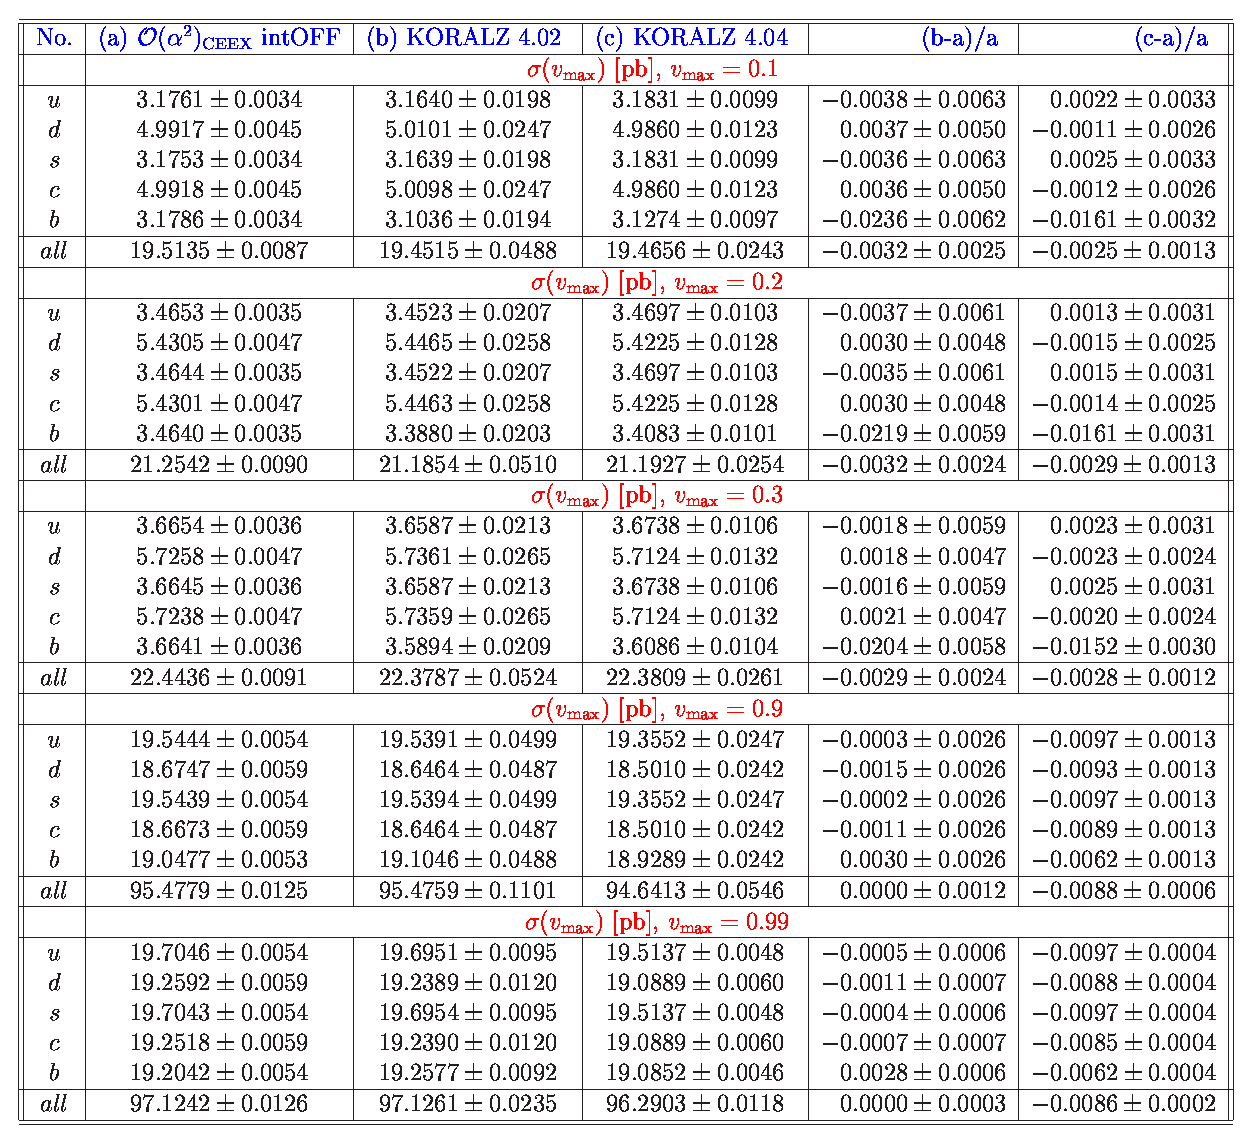
\epsfig{file=tab2wt-189GeV.eps,width=80mm,height=70mm}}}
\end{picture}
\end{center}
\vspace{-2mm}
\noindent
{\large\bf\color{red}
\KK MC agrees with KORALZ 4.02 and 4.04 generally better than 1\%, except $b$ quark.
}
\vfill
\end{slide*}   %%%
%%%%%%%%%%%%%%%%%%


%%%%%%%%%%%%%%%%%%%%%%%%%%%%%%%%%%%%%%%%%%%%%%%%%%%%%%%%%%%%%%%%%%%%%%%%%%%%
%%%%%%%%%%%%%%%%%%%%%%%%%%%%%%%%%%%%%%%%%%%%%%%%%%%%%%%%%%%%%%%%%%%%%%%%%%%%%
%%%%%%%%%%%%%%%%%%%%%%%%%%%%%%%%%%%%%%%%%%%%%%%%%%%%%%%%%%%%%%%%%%%%%%%%%%%%%
                                                         %%%%%%%%%%%%%%%%%%%%
\begin{slide*}
\titbox{{\large\Color{Magenta} Appendix C: \KK MC versus KORALZ 4.02 and 4.04}}
\noindent
{\large\bf\color{blue}
WT=1 events. $\sqrt{s}$= 189GeV. FSR is off.\\
\KK MC: inclusive run $q=d,u,s,c,b$. \\
The only cut $v=1-s'/s<v_{\max}$.
}
\begin{center}
\setlength{\unitlength}{1mm}
\begin{picture}(80,65)
%#####\put(0,0){\framebox( 65,60){ }}
\put(0,0){\makebox(0,0)[lb]{\epsfig{file=tab2-189GeV.eps,width=80mm,height=70mm}}}
\end{picture}
\end{center}
\vspace{-2mm}
\noindent
{\bf\color{red}
\KK MC agrees with KORALZ 4.02 and 4.04 generally better than 1\%.}
{\bf\color{red} Possible 1.5\% problem for $b$-quark?}
\vfill
\end{slide*}   %%%
%%%%%%%%%%%%%%%%%%




\end{document}



%%%%%%%%%%%%%%%%%%%%%%%%%%%%%%%%%%%%%%%%%%%%%%%%%%%%%%%%%%%%%%%%%%%%%%%%%%%%%
%%%%%%%%%%%%%%%%%%%%%%%%%%%%%%%%%%%%%%%%%%%%%%%%%%%%%%%%%%%%%%%%%%%%%%%%%%%%%
%%%%%%%%%%%%%%%%%%%%%%%%%%%%%%%%%%%%%%%%%%%%%%%%%%%%%%%%%%%%%%%%%%%%%%%%%%%%%
\begin{slide*}                                                %%%%%%%%%%%%%%%
\titbox{{\large\Color{Magenta} Virtual pairs from \KK MC }}
{\color{blue}
\noindent
X-sections for $\mu^+\mu^-$ at 189GeV.\\
Without and with virtual correction due to pair.\\
Virt. pairs are all leptons and quarks, in IS and FS.\\
70\% of correction is due to electron pair.\\
QED ISR, FSR and IFI is on.\\
Simple cut $v=1-M^2_{inv}/s<v_{\max}$. Workshop input.\\
}

\begin{center}
\setlength{\unitlength}{1mm}
\begin{picture}(70,50)
%#####\put(0,0){\framebox( 65,60){ }}
\put(0,0){\makebox(0,0)[lb]{\epsfig{file=TabPair-1.eps,width=70mm,height=50mm}}}
\end{picture}
\end{center}
\vspace{1mm}
\noindent
{\color{red} Remarks: ??
}
\vfill
\end{slide*}   %%%
%%%%%%%%%%%%%%%%%%


\end{document}

